\pdfsuppresswarningpagegroup=1

\documentclass{beamer}
\usetheme{Boadilla}
\usecolortheme{seahorse}
\usepackage{pifont}
\usepackage{svg}
\usepackage{t1enc}
\usepackage[hungarian]{babel}

\titlegraphic{
\includegraphics[width=2cm]{elte_cimer_szines}}
\title[HoloDB]{HoloDB: szintetikus adatok on-the-fly szolgáltatása relációs adatbázisként}
\author[Horváth Dávid]{Horváth Dávid \\ ~ \\ { \footnotesize Témavezető: Dr. Vincellér Zoltán, Mesteroktató }}
\institute[ELTE-IK]{ELTE Informatikai Kar, Információs Rendszerek Tanszék}
\date{2023}


\newcommand{\condpause}{\pause}
%\newcommand{\condpause}{}

\newcommand{\slidetitle}[2]{\frametitle{{\small #1 ~ \ding{226} ~ } #2}}

\begin{document}
\beamertemplatenavigationsymbolsempty

\frame{\titlepage}

\AtBeginSection[]
{
    \begin{frame}
        \frametitle{Tartalom}
        \tableofcontents[currentsection]
    \end{frame}
}

\def\sectiontitle{Motiváció}
\section{\sectiontitle}

\begin{frame}
    \slidetitle{\sectiontitle}{TODO}
    TODO
\end{frame}

\def\sectiontitle{A megoldás váza}
\section{\sectiontitle}

\begin{frame}
    \slidetitle{\sectiontitle}{Általános kétfázisú értékkiosztás}
    
    \centering
    
    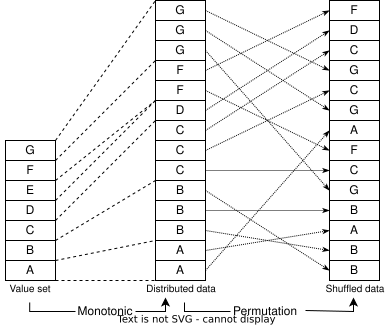
\includegraphics[height=0.5\textwidth]{diagram/distribution}
    
    Kétfázisú értékkiosztás alapelve: \par
    visszafejthető disztribúció és permutáció kompozíciója
\end{frame}

\begin{frame}
    \slidetitle{\sectiontitle}{Kétfázisú értékkiosztás: adatlekérés}
    
    \centering
    
    \includegraphics[height=0.45\textwidth]{diagram/getvalue-0}
    
    \hspace{0.7cm}
    
    Adatlekérés a kétfázisú értékkiosztásból
\end{frame}

\begin{frame}[noframenumbering]
    \slidetitle{\sectiontitle}{Kétfázisú értékkiosztás: adatlekérés}
    
    \centering
    
    \includegraphics[height=0.45\textwidth]{diagram/getvalue-1}
    
    \hspace{0.7cm}
    
    Adatlekérés a kétfázisú értékkiosztásból
\end{frame}

\begin{frame}[noframenumbering]
    \slidetitle{\sectiontitle}{Kétfázisú értékkiosztás: adatlekérés}
    
    \centering
    
    \includegraphics[height=0.45\textwidth]{diagram/getvalue-2}
    
    \hspace{0.7cm}
    
    Adatlekérés a kétfázisú értékkiosztásból
\end{frame}

\begin{frame}[noframenumbering]
    \slidetitle{\sectiontitle}{Kétfázisú értékkiosztás: adatlekérés}
    
    \centering
    
    \includegraphics[height=0.45\textwidth]{diagram/getvalue-3}
    
    \hspace{0.7cm}
    
    Adatlekérés a kétfázisú értékkiosztásból
\end{frame}

\begin{frame}[noframenumbering]
    \slidetitle{\sectiontitle}{Kétfázisú értékkiosztás: adatlekérés}
    
    \centering
    
    \includegraphics[height=0.45\textwidth]{diagram/getvalue-4}
    
    \hspace{0.7cm}
    
    Adatlekérés a kétfázisú értékkiosztásból
\end{frame}

\begin{frame}
    \slidetitle{\sectiontitle}{Kétfázisú értékkiosztás: keresés}
    
    \centering
    
    \includegraphics[height=0.45\textwidth]{diagram/findvalue-0}
    
    \vspace{0.5cm}
    
    Keresés a kétfázisú értékkiosztásban: \par
    A megfordíthatóság biztosítja a hatékony keresést
\end{frame}

\begin{frame}[noframenumbering]
    \slidetitle{\sectiontitle}{Kétfázisú értékkiosztás: keresés}
    
    \centering
    
    \includegraphics[height=0.45\textwidth]{diagram/findvalue-1}
    
    \vspace{0.5cm}
    
    Keresés a kétfázisú értékkiosztásban: \par
    A megfordíthatóság biztosítja a hatékony keresést
\end{frame}

\begin{frame}[noframenumbering]
    \slidetitle{\sectiontitle}{Kétfázisú értékkiosztás: keresés}
    
    \centering
    
    \includegraphics[height=0.45\textwidth]{diagram/findvalue-2}
    
    \vspace{0.5cm}
    
    Keresés a kétfázisú értékkiosztásban: \par
    A megfordíthatóság biztosítja a hatékony keresést
\end{frame}

\begin{frame}[noframenumbering]
    \slidetitle{\sectiontitle}{Kétfázisú értékkiosztás: keresés}
    
    \centering
    
    \includegraphics[height=0.45\textwidth]{diagram/findvalue-3}
    
    \vspace{0.5cm}
    
    Keresés a kétfázisú értékkiosztásban: \par
    A megfordíthatóság biztosítja a hatékony keresést
\end{frame}

\begin{frame}
    \slidetitle{\sectiontitle}{TODO}
    TODO
\end{frame}


\end{document}
